\chapter{Introduzione}
\label{chap:Introduzione}

\section{Ambito della tesi}
\label{sec:ambito della tesi}

Il presente lavoro ha come oggetto lo studio dello sviluppo e della progettazione della piattaforma OVL Dashboard, un portale che permette la gestione e il monitoraggio di una rete virtuale di dispositivi situati in diverse strutture sanitarie su tutto il territorio italiano. Questo progetto è stato realizzato all’interno dell’azienda Themis, durante il mio stage curricolare. Esso ha richiesto, tenendo conto dello studio delle tecnologie per me nuove e dell'effettiva implementazione, circa tre mesi.
Il sito è accessibile a chiunque possegga un account registrato alla piattaforma, la cui creazione avviene tramite invito. Un utente registrato può accedere alle macchine collegate alla rete OVL, modificarne le proprietà o interagire con altri utenti in base ai permessi da esso posseduti. Il portale è accessibile da qualsiasi dispositivo con interfacce semplificate  rendendo il suo uso intuitivo anche a chi possiede scarse competenze digitali.
\newline
Ho scelto, dall’elenco delle proposte di stage disponibili proprio questa in quanto, il mio interesse è rivolto alle tecnologie che permettono la migrazione in cloud di servizi di uso quotidiano. Inoltre, questo stage mi offriva la possibilità di applicare concretamente le mie competenze di full-stack developer e di svilupparle in un contesto lavorativo.
Per la realizzazione di tale progetto ho utilizzato diverse tecnologie tra le quali JavaScript in particolare la libreria ReactJS, NodeJS, MySQL, MongoDB, Git.

\section{Descrizione dell'azienda}
\label{sec:descrizione dell'azienda}

La società Themis s.r.l.\footnote{Themis s.r.l.: \url{http://www.themis.it/}} nasce nell’incubatore del Politecnico di Torino nell’anno 2004, come evoluzione di realtà professionali e da altre società che hanno come filo conduttore l’attività d’ingegneria del software, nata come UNO s.r.l. nel 1981. Dalla sua nascita, Themis interviene nell’organizzazione e management di progetti per l’automazione di sistemi complessi su specifiche che non hanno riscontro in soluzioni pronte nel settore I.T. e nella  raccolta, distribuzione e gestione di dati e condivisione delle risorse, integrando i propri prodotti con le tecnologie più innovative che utilizzano il cloud come naturale centro nodale delle proprie piattaforme.
\newline
I servizi offerti dalla Themis s.r.l. sono il sistema PhC3 e la piattaforma Openvirtuallab (OVL). PhC3 è un’applicazione web basata su sistemi di misura wireless, WiFi o rete mobile, che registra e controlla in continuo le condizioni ambientali di temperatura, umidità relativa, e pressione differenziale dei frigo e dei contenitori per il sangue e gli emoderivati.
OVL, invece, è la piattaforma che verrà trattata nel corso di questo lavoro.

\newpage
\section{Architettura generale del progetto}
\label{sec:architettura generale del progetto}

\begin{figure}
\begin{center}
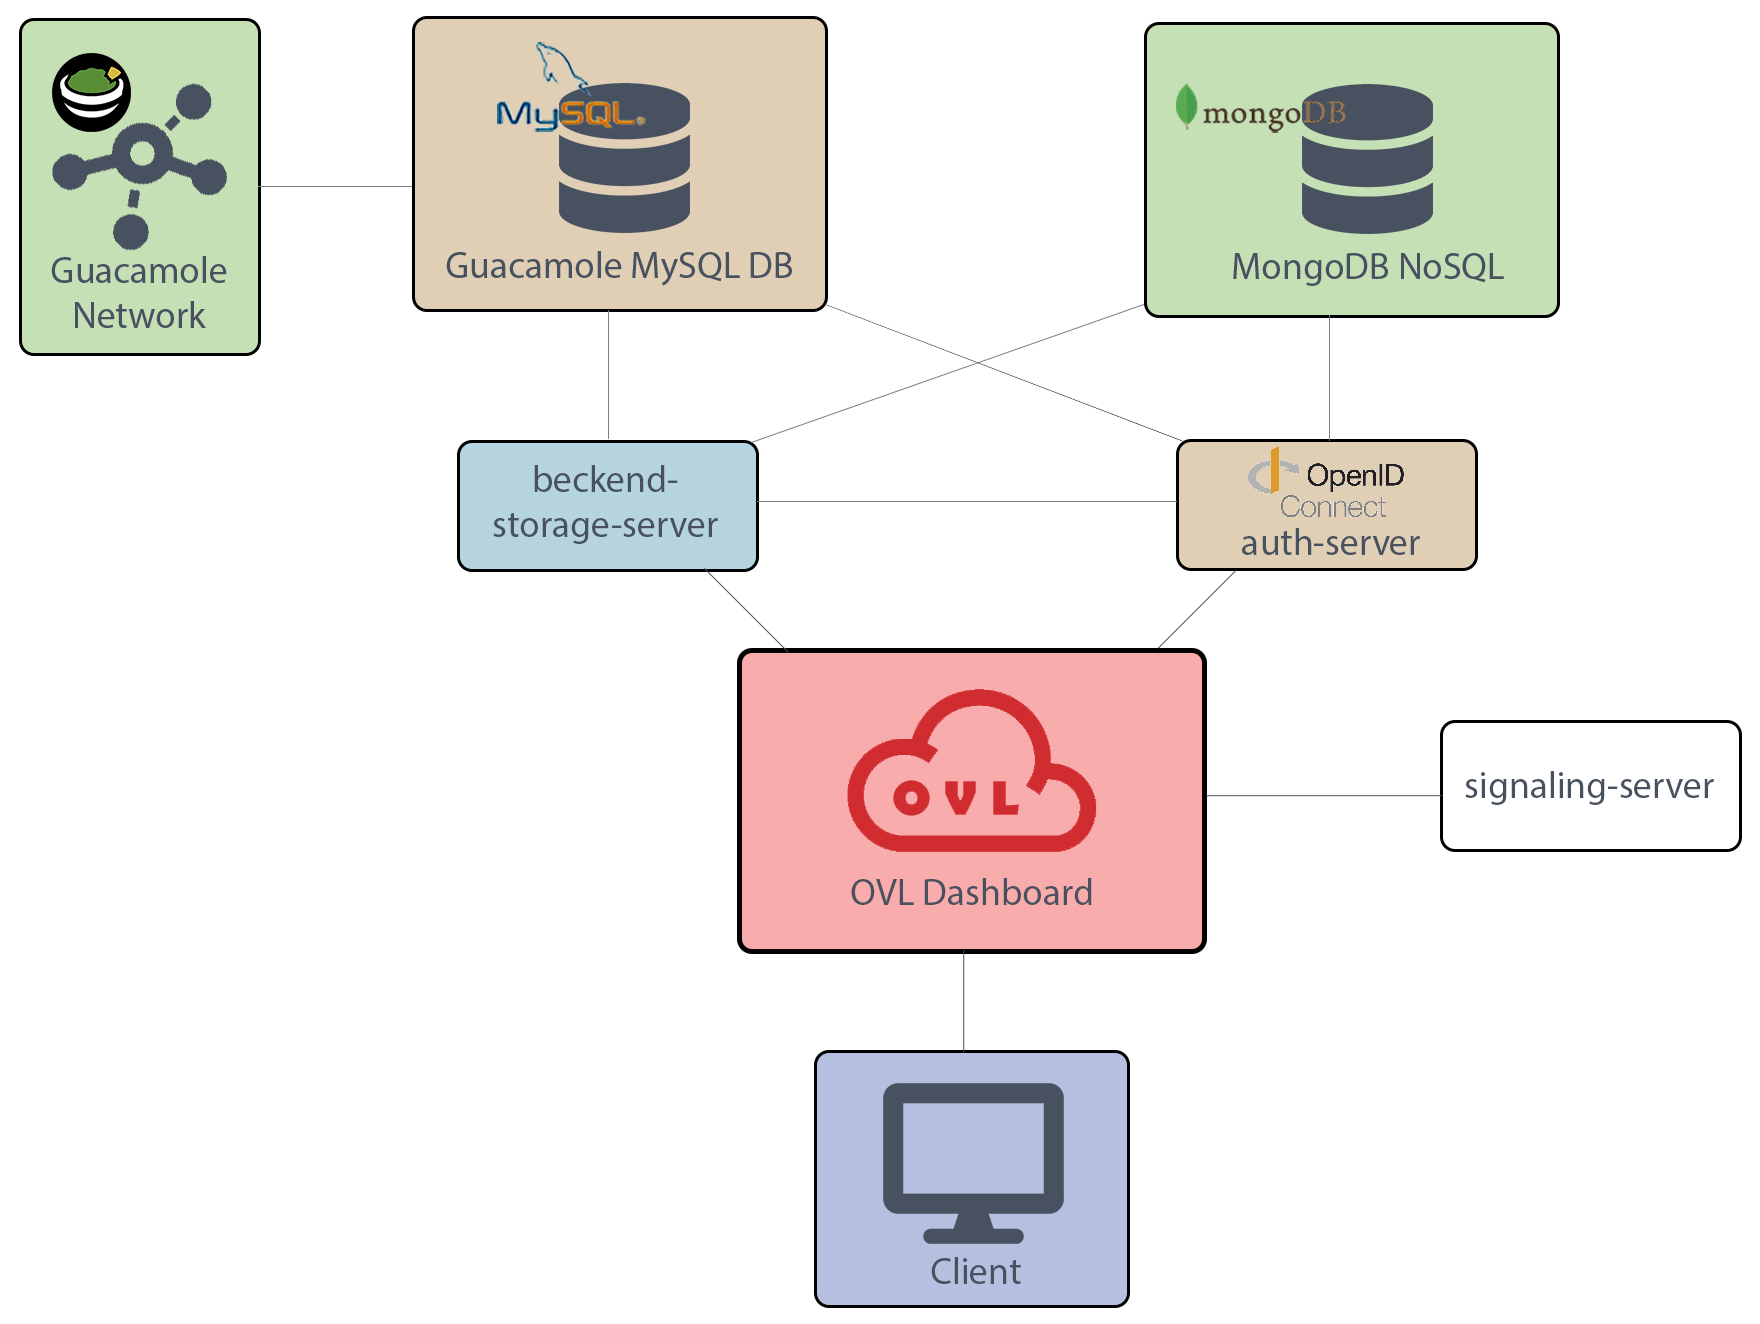
\includegraphics[scale=0.2]{main/images/schema-ovl.jpg}
\end{center}
\caption{Diagramma dell'architettura di OpenVirtualLab.}
\label{fig:schema-ovl}
\end{figure}

L'architettura è composta da:
\begin{itemize}
    \item client browser web: utile agli utenti della piattaforma per interfacciarsi ai servizi forniti da OVL
    \item OVL Dashboard: web application che fornisce un'interfaccia utente sviluppata in JavaScript, in particolare utilizzando la libreria ReactJS\footnote{ReactJS: \url{https://it.reactjs.org/}} e ReduxJS\footnote{ReduxJS: \url{https://redux.js.org/}}
    \item backend-storage-server (ExpressJS\footnote{ExpressJS: \url{https://expressjs.com/}}, framework di creazione di API basato su NodeJS): mette a disposizione gli endpoint API richiamabili dal client, accede al database MySQL per interagire con le connessioni appartenenti alla rete di Guacamole
    \item auth-server (ExpressJS): è un server di autorizzazione OAuth 2.0 basato su OpenID Connect\footnote{OpenID Connect: \url{https://openid.net/connect/}} e fornisce gli endpoint per la gestione degli account registrati alla piattaforma
    \item signal-server (WebSocketServer): server di segnalazione che permette ai client di connettersi e fare segnalazioni per la comunicazione mediante WebRTC\footnote{WebRTC: \url{https://webrtc.org/}}
    \item Guacamole database (MySQL\footnote{MySQL: \url{https://www.mysql.com/}}): necessario per memorizzare le informazioni riguardanti le connessioni della rete di Guacamole ed i relativi utenti 
    \item database NoSQL (MongoDB\footnote{MongoDB: \url{https://www.mongodb.com/}}): necessario per memorizzare le informazioni riguardanti gli utenti registrati presso il server di autorizzazione
    \item rete Guacamole\footnote{Guacamole: \url{https://guacamole.apache.org/}}: fornisce l'accesso agli ambienti desktop mediante protocolli desktop remoti (come VNC o RDP)
\end{itemize}

\section{Obiettivo del progetto}
\label{sec:obiettivo del progetto}

L'obiettivo del progetto è quello di sviluppare una piattaforma che sia in grado di offrire all'utente un mezzo per la gestione e il monitoraggio delle connessioni remote a dispositivi collocati in diverse strutture sanitarie. Inoltre, permette agli utenti di comunicare in tempo reale tra di essi. Questa funzionalità trova spazio d'utilizzo, ad esempio, nel caso in cui un medico necessiti di una consulenza da parte di uno specialista rispetto a determinate problematiche cliniche. 
Durante la realizzazione del progetto, mi sono occupato dello sviluppo delle pagine della dashboard relative alla creazione, alla modifica e all'eliminazione delle connessioni,  alla differenziazione dei vari livelli e tipologie di utenti e le conseguenti differenze legate all'interfaccia e alle operazioni che essi possono eseguire. Inoltre, mi sono occupato della creazione e della modifica degli endpoint nello storage server e della modifica degli endpoint del server di autorizzazione, relativi alla registrazione e al login, rispettando ovviamente l'architettura precedentemente descritta.
\newline
Un altro aspetto del progetto di cui mi sono occupato è stato quello dello studio e dell'implementazione iniziale di una pagina che permetta l'interazione real-time fra utenti della piattaforma utilizzando le API web della libreria WebRTC.